\section{Test setup}\label{ssec:test_setup}
To characterise the performance of the linoSPAD under radiation, a test was performed in the cylcotron of the Paul Screrrer Institute (PSI) in Switzerland. The test involved proton radiation beams of both $60\,MeV$ and $10.1\,MeV$. A schematic of the setup is shown in \cref{tkz:test_setup}. The collimator and radiation shield have to make sure that only the SPAD array gets a large radiation dose. \Cref{fig:dosis} shows the amount of radiation that is projected onto the SPAD array as a function of time. The red dashed lines indicate the start and stop time of the $60\,MeV$ beam, and the green dashed lines indicate the start and stop of the $10\,MeV$ beam. The collimator eeds to be replaced when switching from $60\,MeV$ to $10\,MeV$ which is why the power of the SPAD array will be off for a brief time during the test. The blue line indicates the moment the power of the SPAD array is off.

\begin{figure}[H]
    \centering



\begin{tikzpicture}

\draw  (-6,-5.5) rectangle (5,-6) node[pos=.5]{circuitboard};
\draw  (0,-5) rectangle (4.5,-5.5)node[pos=.5]{ROIC and FPGA};
\draw  (-4.5,-5) rectangle (-2.5,-5.5)node[pos=.5]{SPADs};

\draw (5.5,-4) -- (-1,-4) -- (-1,-2.5) -- (5.5,-2.5);

\node at (2.5,-3.25) {radiation shield};

\draw [>=latex, ->] (-3.5,2) -- (-3.5,-5);
\node at (-3.5,2.5) {proton beam};
\draw  (-8.5,0) rectangle (-3.75,-1) node[pos=.5]{collimator};
\draw  (-3.25,0) rectangle (1.5,-1) node[pos=.5]{collimator};

\draw [>=latex, ->] (-3.6,2) -- (-3,0);
\draw [>=latex, ->] (-3.7,2) -- (-3.8,0);
\draw [>=latex, ->] (-3.4,2) -- (-3.75,-.5);
\draw [>=latex, ->] (-3.45,2) -- (-3.65,-5);

\end{tikzpicture}


    \caption{schematic of radiation test setup}
    \label{tkz:test_setup}
\end{figure}




\begin{figure}[h]
\centering
	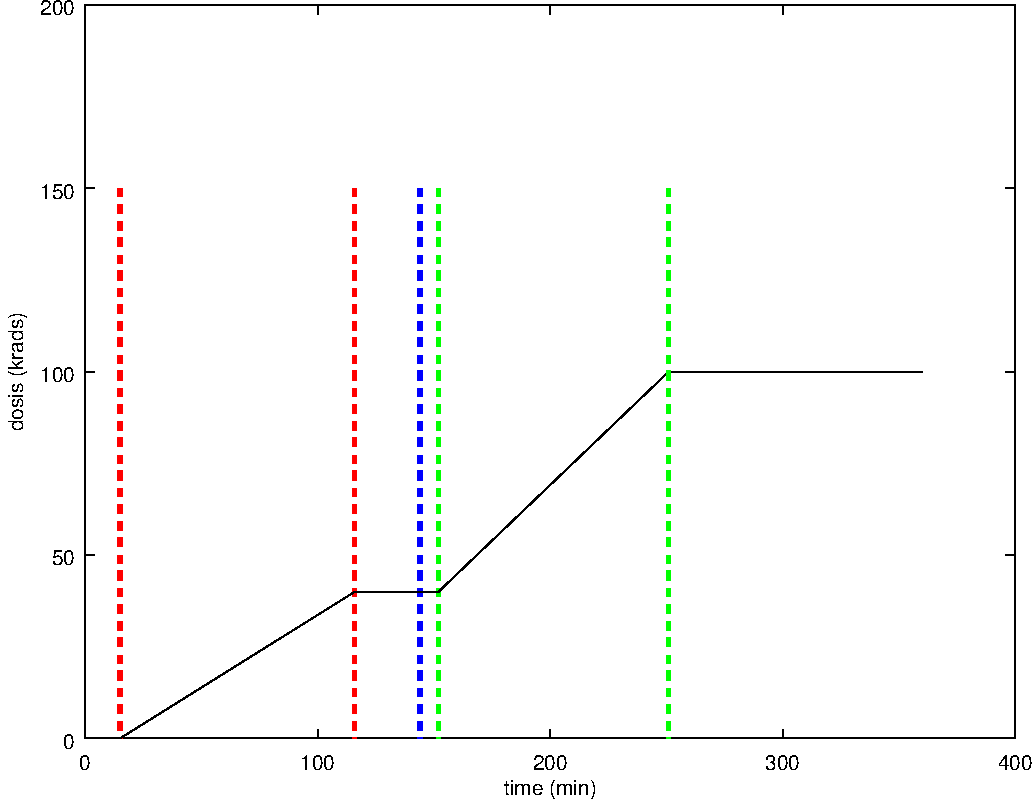
\includegraphics[width=0.6\linewidth]{fig/dosis.pdf}
\caption{The accumulative dose of radiation produces by the proton radiance as a function of time}
\label{fig:dosis}
\end{figure}


